% Copyright 2004 by Till Tantau <tantau@users.sourceforge.net>.
%
% In principle, this file can be redistributed and/or modified under
% the terms of the GNU Public License, version 2.
%
% However, this file is supposed to be a template to be modified
% for your own needs. For this reason, if you use this file as a
% template and not specifically distribute it as part of a another
% package/program, I grant the extra permission to freely copy and
% modify this file as you see fit and even to delete this copyright
% notice. 

\documentclass[xcolor=table]{beamer}
\usepackage{menukeys}[os=win]
\usepackage{textcomp}
\usepackage{tcolorbox}
\usepackage{listings}
\lstset{
  basicstyle=\tiny\ttfamily,
}

% There are many different themes available for Beamer. A comprehensive
% list with examples is given here:
% http://deic.uab.es/~iblanes/beamer_gallery/index_by_theme.html
% You can uncomment the themes below if you would like to use a different
% one:
%\usetheme{AnnArbor}
%\usetheme{Antibes}
%\usetheme{Bergen}
%\usetheme{Berkeley}
%\usetheme{Berlin}
%\usetheme{Boadilla}
%\usetheme{boxes}
%\usetheme{CambridgeUS}
%\usetheme{Copenhagen}
%\usetheme{Darmstadt}
%\usetheme{default}
%\usetheme{Frankfurt}
%\usetheme{Goettingen}
%\usetheme{Hannover}
%\usetheme{Ilmenau}
\usetheme{JuanLesPins}
%\usetheme{Luebeck}
%\usetheme{Madrid}
%\usetheme{Malmoe}
%\usetheme{Marburg}
%\usetheme{Montpellier}
%\usetheme{PaloAlto}
%\usetheme{Pittsburgh}
%\usetheme{Rochester}
%\usetheme{Singapore}
%\usetheme{Szeged}
%\usetheme{Warsaw}
\setbeamerfont{block body}{size=\small}
\title{KF5004 - Subdomains}
\titlegraphic{
\includegraphics[width=0.3\textwidth]{../images/logo.png}}


% A subtitle is optional and this may be deleted
% \subtitle{(Using proximity detection)}

\author{Dr.~Neil~Eliot \& Dr.~Alun~Moon}
% - Give the names in the same order as the appear in the paper.
% - Use the \inst{?} command only if the authors have different
%   affiliation.

%\renewcommand\appendixname{Appendix}

\institute[Northumbria University] % (optional, but mostly needed)
{
  Department of Computer and Information Sciences\\
  University of Northumbria
  % \and
  % \inst{2}
  % Department of Theoretical Philosophy\\
  % University of Elsewhere
}
% - Use the \inst command only if there are several affiliations.
% - Keep it simple, no one is interested in your street address.

\date{Session 7}
% - Either use conference name or its abbreviation.
% - Not really informative to the audience, more for people (including
%   yourself) who are reading the slides online

\subject{Introduction}
% This is only inserted into the PDF information catalog. Can be left
% out. 

% If you have a file called "university-logo-filename.xxx", where xxx
% is a graphic format that can be processed by latex or pdflatex,
% resp., then you can add a logo as follows:

% \pgfdeclareimage[height=0.5cm]{university-logo}{university-logo-filename}
% \logo{\pgfuseimage{university-logo}}

% Delete this, if you do not want the table of contents to pop up at
% the beginning of each subsection:
% \AtBeginSubsection[]
% {
%   \begin{frame}<beamer>{Outline}
%     \tableofcontents[currentsection,currentsubsection]
%   \end{frame}
% }

% Let's get started

\begin{document}

\begin{frame}
  \titlepage
\end{frame}

\begin{frame}{Introduction}
  \tableofcontents
  % You might wish to add the option [pausesections]
\end{frame}

% Section and subsections will appear in the presentation overview
% and table of contents.

\section{Introduction}
\subsection{Background}
\begin{frame}{\texttt{DNS} Subdomains}
  \begin{itemize}
    \item Domain names are generally setup as a \texttt{TLD}, \texttt{SLD} and a \texttt{subdomain}.
      \begin{itemize}
        \item i.e. \texttt{www.example.com.}
      \end{itemize}
    \item Generally the final part, \texttt{www}, is the full address and is simply referred to as the \texttt{domain name} or \texttt{FQDN}.
    \item \texttt{Subdomain}s are created by extending the final part of the \texttt{domain name} further.
      \begin{itemize}
        \item i.e \texttt{www.finance.example.com.}
      \end{itemize}
  \end{itemize}
\end{frame}

\begin{frame}{Why have \texttt{subdomain}s?}
  \begin{itemize}
    \item \texttt{Subdomain}s create a greater scope of \texttt{domain names} within an organisation.
    \item Allow responsibility of \texttt{domain} management to be delegated to multiple administrators.
    \begin{itemize}
      \item i.e. Reduces the workload of the \texttt{DNS} administrator.
    \end{itemize}
  \end{itemize}
\end{frame}

\section{Deployment strategies}
\subsection{Management}
\begin{frame}{Full and Pseudo delegation}
  \begin{itemize}
    \item \textbf{Fully delegated \texttt{subdomains}}
      \begin{itemize}
        \item Requires multiple servers
        \item The delegated administrator has complete control of the \texttt{subdomain} server.
      \end{itemize}
    \item \textbf{Pseudo delegated \texttt{subdomains}}
      \begin{itemize}
        \item Requires only a single server
        \item All \texttt{subdomains} are part of a single zone.
        \item \texttt{includes} split the zone file into multiple files to provide pseudo delegation 
      \end{itemize}
  \end{itemize}
\end{frame}

\subsection{Full Delegation}
\begin{frame}{Fully delegated \texttt{subdomain}}
  \begin{figure}
    \begin{center}
      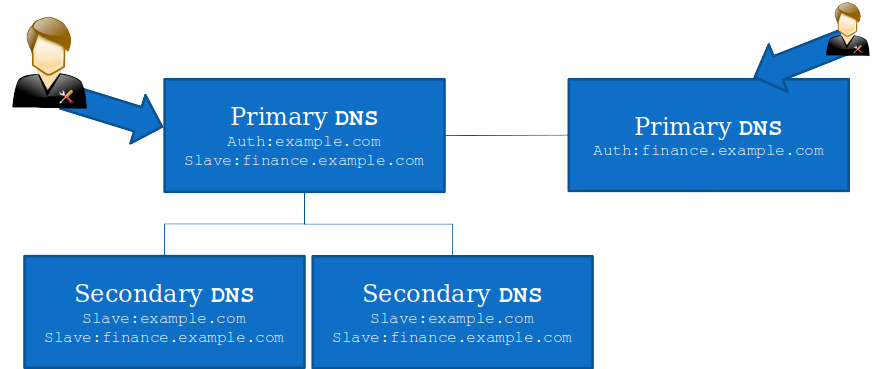
\includegraphics[width=1\linewidth]{FullyDelegated.png}
    \end{center}
  \end{figure}
  \begin{tcolorbox}
    \begin{center}
      \scriptsize Using the \texttt{allow-transfer();} clause. A \texttt{slave} can propagate a \texttt{zone} to another \texttt{slave} and the server will still provide \texttt{authoritative} results.
    \end{center}
  \end{tcolorbox}
\end{frame}

\begin{frame}{Fully delegated \texttt{subdomain}}
  \begin{figure}
    \begin{center}
      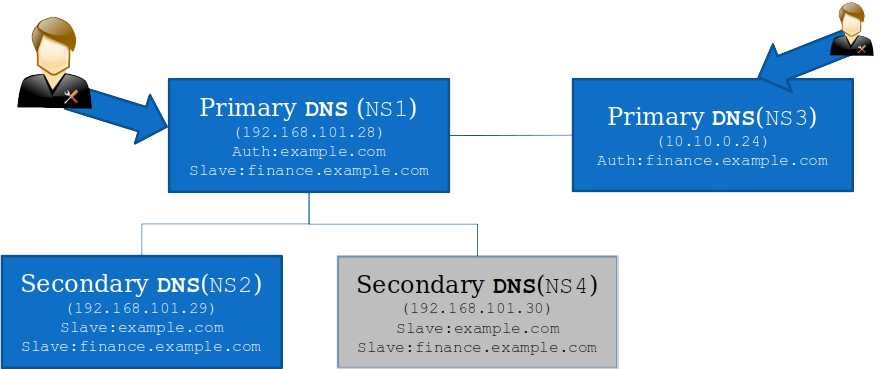
\includegraphics[width=1\linewidth]{FullyDelegated2.png}
    \end{center}
  \end{figure}
  \begin{tcolorbox}
    \begin{center}
      \scriptsize Using the \texttt{allow-transfer();} clause. A \texttt{slave} can propagate a \texttt{zone} to another \texttt{slave} and the server will still provide \texttt{authoritative} results.
    \end{center}
  \end{tcolorbox}
\end{frame}

\begin{frame}[fragile]{Primary \texttt{DNS} (\texttt{NS1}) \texttt{named.conf.local}}
  \begin{tcolorbox}
    \lstset{
      basicstyle=\tiny\ttfamily,
    }
    \begin{lstlisting}
      zone "example.com" IN {
	      type master;
	      file "/etc/bind/db.example.com";
	      allow-transfer{192.168.101.29; 192.168.101.30;};
      };
      // NS1 acts as the slave (secondary) for 
      // the delegated subdomain
      zone "finance.example.com" IN {
	      type slave;
	      file "db.finance.example.com";
	      masters{10.10.0.24;};
	      allow-transfer{192.168.101.29; 192.168.101.30;};
      };    
    \end{lstlisting}
  \end{tcolorbox}
\end{frame}

\begin{frame}[fragile]{Primary \texttt{DNS} (\texttt{NS1}) \texttt{db.example.com}}
  \begin{tcolorbox}
    \lstset{
      basicstyle=\tiny\ttfamily,
    }
    \begin{lstlisting}
      $TTL 2d ; default TTL is 2 days
      $ORIGIN example.com.
      @ . IN SOA example.com. hostmaster.example.com. (
	              2020032723 ; serial number
	              12h ; refresh = 12 hours
	              15m ; refresh retry = 15 minutes
	              3w12h ; expiry = 3 weeks + 12 hours
	              2h20m ; nx = 2 hours + 20 minutes
                )
      ; main domain name servers
	          IN NS 	ns2.example.com.
	          IN NS 	ns4.example.com.
      ns2 	IN A 	  192.168.101.29
      ns4 	IN A 	  192.168.101.30
…
    \end{lstlisting}
  \end{tcolorbox}
\end{frame}

\begin{frame}[fragile]{Primary \texttt{DNS} (\texttt{NS3}) \texttt{named.conf.local}}
  \begin{tcolorbox}
    \lstset{
      basicstyle=\tiny\ttfamily,
    }
    \begin{lstlisting}
      zone "finance.example.com" IN {
	        type master;
	        file "/etc/bind/db.finance.example.com";
	        allow-transfer{192.168.101.28;};
      };
    \end{lstlisting}
  \end{tcolorbox}
\end{frame}

\begin{frame}[fragile]{Primary \texttt{DNS} (\texttt{NS3}) \texttt{db.finance.example.com}}
  \begin{tcolorbox}
    \lstset{
      basicstyle=\tiny\ttfamily,
    }
    \begin{lstlisting}
      ; zone file for subdomain finance.example.com
      $TTL 2d ; zone default of 2 days
      $ORIGIN finance.example.com.
      @	IN SOA example.com. hostmaster.example.com. (
              2020122135 ; serial number
              2h ; refresh = 2 hours
              15m ; refresh retry = 15 minutes
              3w12h ; expiry = 3 weeks + 12 hours
              2h20m ; nx = 2 hours + 20 minutes
              )
      ; subdomain name servers
      @			    IN    NS    ns2.example.com.
                IN    NS    ns4.example.com.
      ns3 			IN    A     10.10.0.24
      ftp 			IN    A     10.10.0.28
      ...   
    \end{lstlisting}
  \end{tcolorbox}
\end{frame}

\begin{frame}[fragile]{Secondary \texttt{DNS} (\texttt{NS2}) \texttt{named.conf.local}}
  \begin{tcolorbox}
    \lstset{
      basicstyle=\tiny\ttfamily,
    }
    \begin{lstlisting}
      zone "example.com" IN {
	      type slave;
	      file "db.example.com";
	      masters{192.168.101.27;};
      };
      // NS1 acts as the slave (secondary) for 
      // the delegated subdomain
      zone "finance.example.com" IN {
	      type slave;
	      file "db.finance.example.com";
	      masters{192.168.101.27;};
      };
    \end{lstlisting}
  \end{tcolorbox}
\end{frame}

\subsection{Pseudo Delegation}
\begin{frame}{Pseudo delegated \texttt{subdomain}}
  \begin{figure}
    \begin{center}
      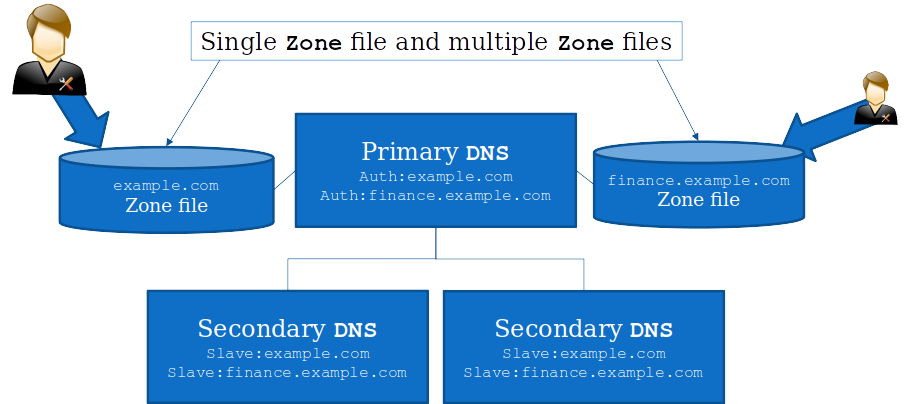
\includegraphics[width=1\linewidth]{PseudoDelegated.png}
    \end{center}
  \end{figure}
\end{frame}

\begin{frame}{Multi-file delegated \texttt{subdomain}}
  \begin{figure}
    \begin{center}
      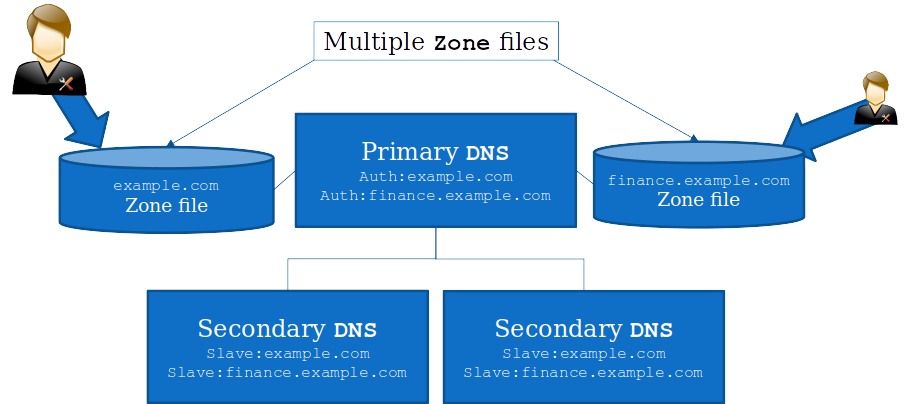
\includegraphics[width=1\linewidth]{MultipleDelegated.png}
    \end{center}
  \end{figure}
\end{frame}

\begin{frame}{Single file delegated \texttt{subdomain}}
  \begin{figure}
    \begin{center}
      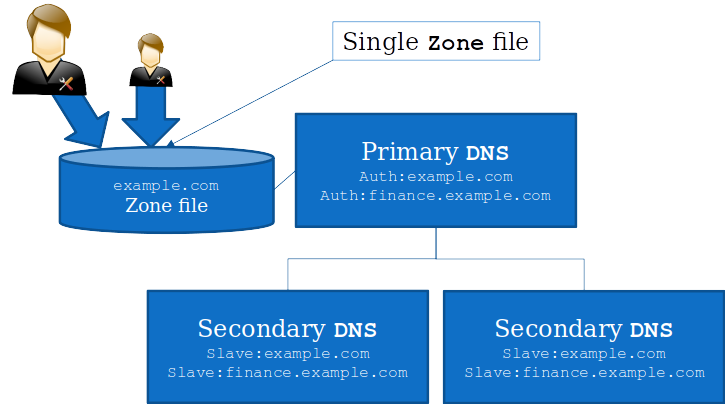
\includegraphics[width=0.8\linewidth]{SingleDelegated.png}
    \end{center}
  \end{figure}
\end{frame}

\begin{frame}[fragile]{Primary \texttt{DNS} \texttt{named.conf.local}}
  \begin{tcolorbox}
    \lstset{
      basicstyle=\tiny\ttfamily,
    }
    \begin{lstlisting}
      zone "example.com" IN {
	      type master;
	      file "/etc/bind/db.example.com";
	      allow-transfer{192.168.101.28; 192.168.101.30};
      };
    \end{lstlisting}
  \end{tcolorbox}
\end{frame}

\begin{frame}[fragile]{Primary \texttt{DNS} \texttt{named.conf.local} (Single file)}
  \begin{tcolorbox}
    \lstset{
      basicstyle=\tiny\ttfamily,
    }
    \begin{lstlisting}
      ; zone fragment for example.com
      $TTL 2d ; zone default = 2 days or 172800 seconds
      $ORIGIN example.com.
      @	      IN SOA example.com. hostmaster.example.com. (
	          2020032723 ; serial number
	          2h ; refresh = 2 hours
	          15M ; refresh retry = 15 minutes
	          3W12h ; expiry = 3 weeks + 12 hours
	          2h20M ; nx = 2 hours + 20 minutes
            )
      ; main domain name servers
		          IN    NS 	ns2.example.com.
		          IN    NS 	ns3.example.com.
      ns2 		  IN    A 	192.168.101.29
      ns3 		  IN    A 	192.168.101.30
      ; subdomain definitions
      $ORIGIN finance.example.com.
      ftp 		  IN    A   10.10.0.29
      www		  IN    A   10.10.0.55
      ...
    \end{lstlisting}
  \end{tcolorbox}
\end{frame}

\begin{frame}[fragile]{Primary \texttt{DNS} \texttt{named.conf.local} (Multi-file)}
  \begin{tcolorbox}
    \lstset{
      basicstyle=\tiny\ttfamily,
    }
    \begin{lstlisting}
      ; zone fragment for example.com
      $TTL 2d ; zone default = 2 days or 172800 seconds
      $ORIGIN example.com.
      @	      IN SOA example.com. hostmaster.example.com. (
                2020032723 ; serial number
                2h ; refresh = 2 hours
                15M ; refresh retry = 15 minutes
                3W12h ; expiry = 3 weeks + 12 hours
                2h20M ; nx = 2 hours + 20 minutes
                )
      ; main domain name servers
                        IN    NS 	ns2.example.com.
                        IN    NS 	ns3.example.com.
      ns2 		IN    A 	192.168.101.29
      ns3 		IN    A 	192.168.101.30
      ; subdomain definitions
      $INCLUDE	db.finance.example.com
      ...
    \end{lstlisting}
  \end{tcolorbox}
\end{frame}

\begin{frame}[fragile]{Primary \texttt{DNS} \texttt{db.finance.example.com} (Multi-file)}
  \begin{tcolorbox}
    \lstset{
      basicstyle=\tiny\ttfamily,
    }
    \begin{lstlisting}
      $ORIGIN finance.example.com.
      ftp 		  IN    A   10.10.0.29
      www		  IN    A   10.10.0.55
      ...
    \end{lstlisting}
  \end{tcolorbox}
\end{frame}

\begin{frame}[fragile]{Secondary \texttt{DNS} \texttt{named.conf.local} (Multi-file)}
  \begin{tcolorbox}
    \lstset{
      basicstyle=\tiny\ttfamily,
    }
    \begin{lstlisting}
      zone "example.com" IN {
	        type slave;
	        file "db.example.com";
	        masters{192.168.101.28;};
      } ;
    \end{lstlisting}
  \end{tcolorbox}
\end{frame}


\section*{Conclusion}
\begin{frame}{Conclusion}
  \begin{itemize}
    \item \texttt{Subdomains} provide an extended \texttt{domain} scope.
    \item \texttt{Subdomains} can be \texttt{fully delegated} but this adds additional server for management.
      \begin{itemize}
        \item However, you can have geographical deployment.
      \end{itemize}
    \item \texttt{Subdomains} can be \texttt{pseudo delegated} but this requires added secuirty measures for implementation.
  \end{itemize}
\end{frame}

\end{document}


